\chapter{Template}\label{ch:template}


\section{Section A}%\label{sec:a}
This is regular text.

\subsection{Section A-1}
This is regular text.

\subsection{Section A-2}
\enquote{And I am a cited text!}\parencite[vgl.][S. 152]{sousa_new_2005}

\subsubsection{Section A-2-i}
\verb|some_file.ending|
This is an \mccorrect{inline} correction (highlighting can be disabled in report.tex).

\begin{mccorrection}
    This is a whole paragraph which is being highlighted.
\end{mccorrection}

Just some \textit{italic} text.
Just some \textbf{bold} text.
Just some \texttt{very bold} text.

\section{Section B}%\label{sec:b}
This is regular text.

\begin{figure}
    \centering
    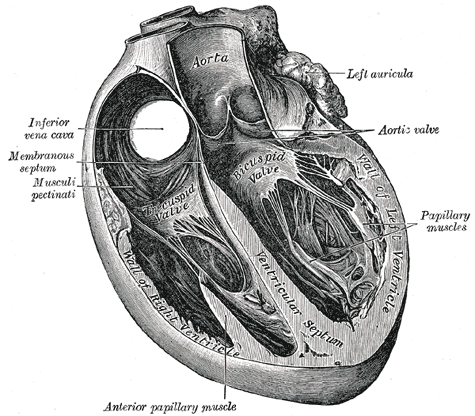
\includegraphics[width=0.7\textwidth]{content/figures/sample/Gray498}
    \caption[I'm the short title for the TOC]{And I'm the caption appearing next to the actucal graphic. So I can be quite extensive, and, even if not very sensible, completely distinct from the TOC variant.}
    \label{fig:heart}
\end{figure}

\begin{code}[H]
    \begin{minted}{py3}
if _algorithm == "MD5" or _algorithm == "MD5-SESS":
    def md5_utf8(x):
        if isinstance(x, str):
            x = x.encode("utf-8")
        return hashlib.md5(x).hexdigest()
    hash_utf8 = md5_utf8
    \end{minted}
    \caption[Verwendung Algorithmus]{Verwendung eines Algorithmus mit extrem langem und nicht ins TOC passendem Titel}
    \label{code:md5}
\end{code}